\documentclass[12pt]{article}
\usepackage[letterpaper, margin=1in]{geometry}
\usepackage{graphicx}
\usepackage{subcaption}
\graphicspath{{./figures/}}
\usepackage{hyperref}
\hypersetup{colorlinks = true}
\usepackage{parskip}
\usepackage{amsmath}
%\usepackage{siunitx}
%\usepackage{pgfplots}
%\usepackage{pgfplotstable}
%\pgfplotsset{compat = newest}
\usepackage{titlesec}
\usepackage{enumitem}
\usepackage{listings}
%\usepackage[framed, numbered]{matlab-prettifier}
\lstset{basicstyle=\small, frame=single, breaklines=true}
\usepackage{longtable}

\titleformat*{\section}{\large\bfseries}
%\allowdisplaybreaks

% remove vertical spacing above top figure
\makeatletter
\setlength{\@fptop}{0pt}
\makeatother
%

\title{COMPENG 4DM4 Assignment 1 Report}
\author{
    Aaron Pinto \\
    pintoa9 \\
    %L02
    \and
    Raeed Hassan \\
    hassam41 \\
    %L02
}

\begin{document}

\maketitle
\clearpage

\section*{Assumptions}
In addition to the assumptions stated in the assignment, the following assumptions are made for all parts of the assignment:
\begin{itemize}
    \item FP-ADD unit 3-stage pipeline labeled as A1, A2, A3
    \item FP-MULT unit 6-stage pipeline labeled as FM1, FM2, FM3, FM4, FM5, FM6
    \item Full forwarding of data from WB stage to any stage
	\item assume dual-ported memory that allows simultaneous read and/or write on two ports
	\item we can perform 2 write-backs per clock cycle
\end{itemize}

\section*{Part (a): DAXPY Loop, No Unrolling, with No Scheduling}
The timing diagram is shown in Figure~\ref{fig:a}. The timing diagram is also submitted as 4DM4-Assignment-\#2a-Basic-Timing-Table.xlsx. The performance, or MFLOP rating, of the implementation with a 3 GHz clock is (3 GHz)*(2 FLOP/19 cc) = 315.8 MFLOP/s.

\begin{figure}[htp]
\centering
\caption{Timing Diagram for DAXPY Loop (No Unrolling, No Scheduling)}
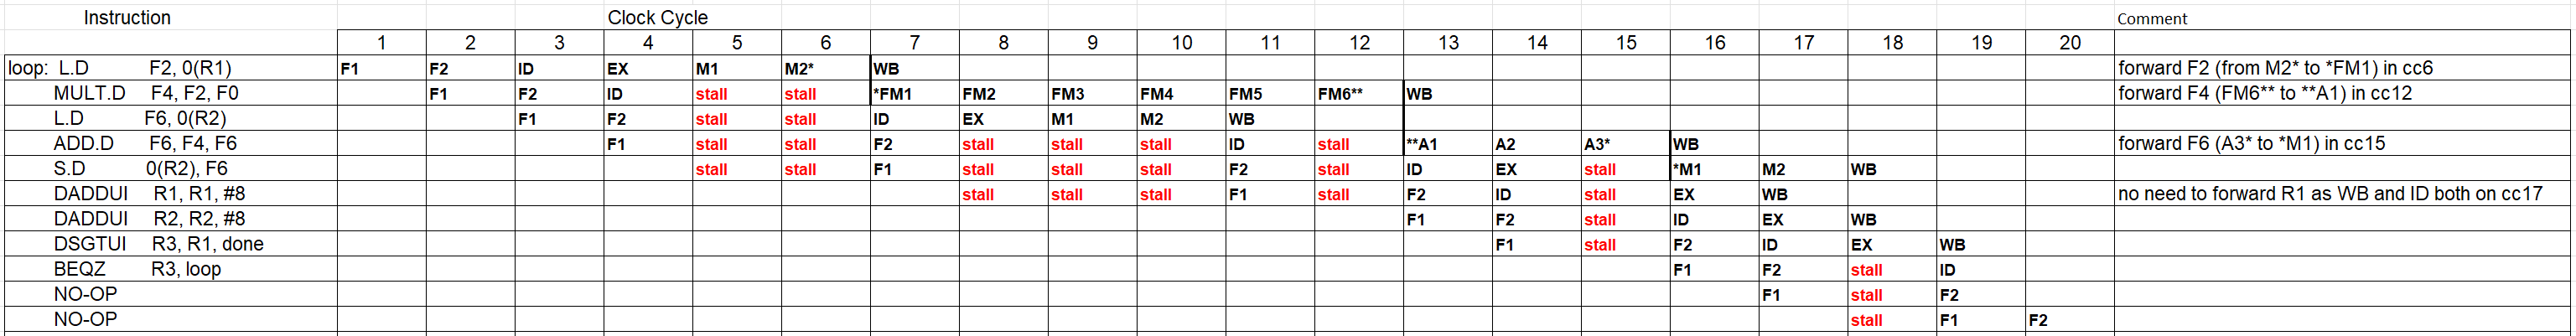
\includegraphics[width=\textwidth]{a.png}
\label{fig:a}
\end{figure}

\section*{Part (b): DAXPY Loop, No Unrolling, with Scheduling}
The timing diagram is shown in Figure~\ref{fig:b}. The timing diagram is also included in the submission as 4DM4-Assignment-\#2b-Basic-Timing-Table-Group-47-RH,AP.xlsx. The performance, or MFLOP rating, of the implementation with a 3 GHz clock is (3 GHz)*(2 FLOP/13 cc) = 461.5 MFLOP/s.

\begin{figure}[htp]
\centering
\caption{Timing Diagram for DAXPY Loop (No Unrolling, Scheduling)}
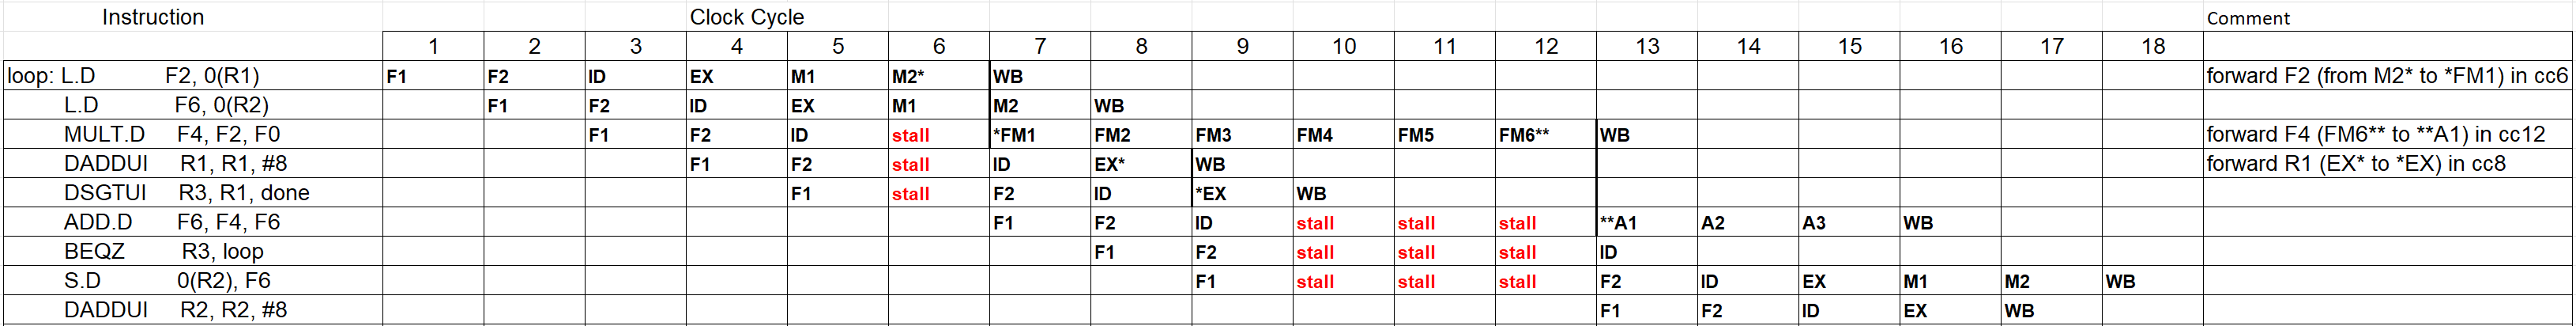
\includegraphics[width=\textwidth]{b.png}
\label{fig:b}
\end{figure}

\section*{Part (c): DAXPY Loop, With Unrolling, with no Scheduling}
The compressed timing diagram is shown in Table~\ref{tab:c}. The compressed timing diagram is also included in the submission as 4DM4-Assignment-\#2c-Compressed-Timing-Table-single-issue-Group-47-RH,AP.xlsx. The performance, or MFLOP rating, of the implementation with a 3 GHz clock is (3 GHz)*(8 FLOP/61 cc) = 393.4 MFLOP/s.

\begin{table}[htp]
\centering
\caption{Compressed Timing Diagram for DAXPY Loop (Unrolling, No Scheduling)}\label{tab:c}
\resizebox{\textwidth}{!}{
\begin{tabular}{|l|c|c|c|c|c|l|}
	\hline
	Instruction   Slot \#1 &
	  IF (F1,F2) &
	  ID &
	  EX (Int, FP) &
	  MEM (M1,M2) &
	  WB &
	  \multicolumn{1}{c|}{Comment/Hazard} \\ \hline
	loop:  L.D            F2, 0(R1) &
	  1,2 &
	  3 &
	  4 &
	  5,6* &
	  7 &
	  forward F2 (from M2* to *FM1) in cc6 \\ \hline
	MULT.D     F4, F2, F0 &
	  2,3 &
	  4 &
	  *7,8,9,10,11,12** &
	   &
	  13 &
	  \begin{tabular}[c]{@{}l@{}}forward   F4 (FM6** to **A1) in cc12\\ stall on FM1 waiting for F2\end{tabular} \\ \hline
	L.D            F6, 0(R2) &
	  3,4 &
	  7 &
	  8 &
	  9,10 &
	  11 &
	   \\ \hline
	ADD.D       F6, F4, F6 &
	  5,7 &
	  11 &
	  **13,14,15* &
	   &
	  16 &
	  \begin{tabular}[c]{@{}l@{}}forward   F6 (A3* to *M1) in cc15\\ stall on ID waiting for F6\\ stall on A1 waiting for F4\end{tabular} \\ \hline
	S.D            0(R2), F6 &
	  7,11 &
	  13 &
	  14 &
	  *16,17 &
	  18 &
	  stall on M1 waiting   for F6 \\ \hline
	DADDUI     R1, R1, \#8 &
	  11,13 &
	  14 &
	  16 &
	   &
	  17 &
	   \\ \hline
	DADDUI     R2, R2, \#8 &
	  13,14 &
	  16 &
	  17 &
	   &
	  18 &
	   \\ \hline
	L.D            F2, 0(R1) &
	  14,16 &
	  17 &
	  18 &
	  19,20* &
	  21 &
	  forward F2 (from M2*   to *FM1) in cc20 \\ \hline
	MULT.D     F4, F2, F0 &
	  16,17 &
	  18 &
	  *21,22,23,24,25,26** &
	   &
	  27 &
	  \begin{tabular}[c]{@{}l@{}}forward   F4 (FM6** to **A1) in cc26\\      stall on FM1 waiting for F2\end{tabular} \\ \hline
	L.D            F6, 0(R2) &
	  17,18 &
	  21 &
	  22 &
	  23,24 &
	  25 &
	   \\ \hline
	ADD.D       F6, F4, F6 &
	  18,21 &
	  25 &
	  **27,28,29* &
	   &
	  30 &
	  \begin{tabular}[c]{@{}l@{}}forward   F6 (A3* to *M1) in cc29\\ stall on ID waiting for F6\\ stall on A1 waiting for F4\end{tabular} \\ \hline
	S.D            0(R2), F6 &
	  21,25 &
	  27 &
	  28 &
	  *30,31 &
	  32 &
	  stall on M1 waiting   for F6 \\ \hline
	DADDUI     R1, R1, \#8 &
	  25,27 &
	  28 &
	  30 &
	   &
	  31 &
	   \\ \hline
	DADDUI     R2, R2, \#8 &
	  27,28 &
	  30 &
	  31 &
	   &
	  32 &
	   \\ \hline
	L.D            F2, 0(R1) &
	  28,30 &
	  31 &
	  32 &
	  33,34* &
	  35 &
	  forward F2 (from M2*   to *FM1) in cc34 \\ \hline
	MULT.D     F4, F2, F0 &
	  30,31 &
	  32 &
	  *35,36,37,38,39,40** &
	   &
	  41 &
	  \begin{tabular}[c]{@{}l@{}}forward   F4 (FM6** to **A1) in cc40\\ stall on FM1 waiting for F2\end{tabular} \\ \hline
	L.D            F6, 0(R2) &
	  31,32 &
	  35 &
	  36 &
	  37,38 &
	  39 &
	   \\ \hline
	ADD.D       F6, F4, F6 &
	  32,35 &
	  39 &
	  **41,42,43* &
	   &
	  44 &
	  \begin{tabular}[c]{@{}l@{}}forward   F6 (A3* to *M1) in cc43\\ stall on ID waiting for F6\\ stall on A1 waiting for F4\end{tabular} \\ \hline
	S.D            0(R2), F6 &
	  35,39 &
	  41 &
	  42 &
	  *44,45 &
	  46 &
	  stall on M1 waiting   for F6 \\ \hline
	DADDUI     R1, R1, \#8 &
	  39,41 &
	  42 &
	  44 &
	   &
	  45 &
	   \\ \hline
	DADDUI     R2, R2, \#8 &
	  41,42 &
	  44 &
	  45 &
	   &
	  46 &
	   \\ \hline
	L.D            F2, 0(R1) &
	  42,44 &
	  45 &
	  46 &
	  47,48* &
	  49 &
	  forward F2 (from M2*   to *FM1) in cc48 \\ \hline
	MULT.D     F4, F2, F0 &
	  44,45 &
	  46 &
	  *49,50,51,52,53,54** &
	   &
	  55 &
	  \begin{tabular}[c]{@{}l@{}}forward   F4 (FM6** to **A1) in cc54\\ stall on FM1 waiting for F2\end{tabular} \\ \hline
	L.D            F6, 0(R2) &
	  45,46 &
	  49 &
	  50 &
	  51,52 &
	  53 &
	   \\ \hline
	ADD.D       F6, F4, F6 &
	  46,49 &
	  53 &
	  **55,56,57* &
	   &
	  58 &
	  \begin{tabular}[c]{@{}l@{}}forward   F6 (A3* to *M1) in cc57\\ stall on ID waiting for F6\\ stall on A1 waiting for F4\end{tabular} \\ \hline
	S.D            0(R2), F6 &
	  49,53 &
	  55 &
	  56 &
	  *58,59 &
	  60 &
	  stall on M1 waiting   for F6 \\ \hline
	DADDUI     R1, R1, \#8 &
	  53,55 &
	  56 &
	  58 &
	   &
	  59 &
	   \\ \hline
	DADDUI     R2, R2, \#8 &
	  55,56 &
	  58 &
	  59 &
	   &
	  60 &
	   \\ \hline
	DSGTUI     R3, R1, done &
	  56,58 &
	  59 &
	  60* &
	   &
	  61 &
	  forward R3 (EX* to   *ID) in cc60 \\ \hline
	BEQZ         R3, loop &
	  58,59 &
	  *61 &
	   &
	   &
	   &
	  stall on ID waiting   for R3 \\ \hline
	NO-OP &
	  59,61 &
	   &
	   &
	   &
	   &
	  branch-delay slot \\ \hline
	NO-OP &
	  61,62 &
	   &
	   &
	   &
	   &
	  branch-delay slot \\ \hline
\end{tabular}
}
\end{table}

\section*{Part (d): DAXPY Loop, With Unrolling, and with Scheduling}
The compressed timing diagram is shown in Table~\ref{tab:d}. The compressed timing diagram is also included in the submission as 4DM4-Assignment-\#2d-Compressed-Timing-Table-single-issue-Group-47-RH,AP.xlsx. The performance, or MFLOP rating, of the implementation with a 3 GHz clock is (3 GHz)*(8 FLOP/24 cc) = 1000 MFLOP/s.

\begin{table}[htp]
\centering
\caption{Compressed Timing Diagram for DAXPY Loop (Unrolling, Scheduling)}\label{tab:d}
\resizebox{\textwidth}{!}{
\begin{tabular}{|l|c|c|c|c|c|l|}
	\hline
	Instruction   Slot \#1  & IF (F1,F2) & ID & EX (Int, FP)       & MEM (M1,M2) & WB & \multicolumn{1}{c|}{Comment/Hazard}      \\ \hline
	loop:  L.D            F1, 0(R1) & 1,2   & 3  & 4                  & 5,6   & 7  &                                         \\ \hline
	L.D            F4, 8(R1)        & 2,3   & 4  & 5                  & 6,7   & 8  &                                         \\ \hline
	L.D            F7, 16(R1)       & 3,4   & 5  & 6                  & 7,8   & 9  &                                         \\ \hline
	L.D            F10, 24(R1)      & 4,5   & 6  & 7                  & 8,9   & 10 &                                         \\ \hline
	L.D            F3, 0(R2)        & 5,6   & 7  & 8                  & 9,10  & 11 &                                         \\ \hline
	L.D            F6, 8(R2)        & 6,7   & 8  & 9                  & 10,11 & 12 &                                         \\ \hline
	L.D            F9, 16(R2)       & 7,8   & 9  & 10                 & 11,12 & 13 &                                         \\ \hline
	L.D            F12, 24(R2)      & 8,9   & 10 & 11                 & 12,13 & 14 &                                         \\ \hline
	MULT.D     F2, F1, F0           & 9,10  & 11 & 12,13,14,15,16,17* &       & 18 & forward   F2 (from FM6* to *A1) in cc17 \\ \hline
	MULT.D     F5, F4, F0           & 10,11 & 12 & 13,14,15,16,17,18* &       & 19 & forward   F5 (from FM6* to *A1) in cc18 \\ \hline
	MULT.D     F8, F7, F0           & 11,12 & 13 & 14,15,16,17,18,19* &       & 20 & forward   F8 (from FM6* to *A1) in cc19 \\ \hline
	MULT.D     F11, F10, F0 & 12,13      & 14 & 15,16,17,18,19,20* &             & 21 & forward   F11 (from FM6* to *A1) in cc20 \\ \hline
	DADDUI     R1, R1, \#32         & 13,14 & 15 & 16*                &       & 17 & forward R1 (from EX*   to *EX) in cc16  \\ \hline
	DSGTUI     R3, R1, done         & 14,15 & 16 & *17                &       & 18 &                                         \\ \hline
	ADD.D       F3, F2, F3          & 15,16 & 17 & *18,19,20          &       & 21 &                                         \\ \hline
	ADD.D       F6, F5, F6          & 16,17 & 18 & *19,20,21          &       & 22 &                                         \\ \hline
	ADD.D       F9, F8, F9          & 17,18 & 19 & *20,21,22          &       & 23 &                                         \\ \hline
	ADD.D       F12, F11, F12       & 18,19 & 20 & *21,22,23          &       & 24 &                                         \\ \hline
	S.D            0(R2), F3        & 19,20 & 21 & 22                 & 23,24 & 25 &                                         \\ \hline
	S.D            8(R2), F6        & 20,21 & 22 & 23                 & 24,25 & 26 &                                         \\ \hline
	S.D            16(R2), F9       & 21,22 & 23 & 24                 & 25,26 & 27 &                                         \\ \hline
	BEQZ         R3, loop           & 22,23 & 24 &                    &       &    &                                         \\ \hline
	S.D            24(R2), F12      & 23,24 & 25 & 26                 & 27,28 & 29 &                                         \\ \hline
	DADDUI     R2, R2, \#32         & 24,25 & 26 & 27                 &       & 28 &                                         \\ \hline
\end{tabular}
}
\end{table}

\section*{Part (e): DAXPY Loop, With Unrolling and Scheduling. On Dual-Issue Machine}

The compressed timing diagram is shown in Table~\ref{tab:e}. The compressed timing diagram is also included in the submission as 4DM4-Assignment-\#2e-Compressed-Timing-Table-dual-issue-Group-47-RH,AP.xlsx. The performance, or MFLOP rating, of the implementation with a 3 GHz clock is (3 GHz)*(8 FLOP/16 cc) = 1500 MFLOP/s.

\begin{table}[b]
\centering
\caption{Compressed Timing Diagram for DAXPY Loop (Unrolling, Scheduling, Dual Issue)}\label{tab:e}
\resizebox{0.95\textwidth}{!}{
\begin{tabular}{|l|l|c|c|c|c|c|c|c|c|l|}
	\hline
	\multicolumn{1}{|c|}{Instruction   Slot \#1} &
	  \multicolumn{1}{c|}{Instruction   Slot \#2} &
	  IF &
	  ID &
	  EX1 &
	  MEM1 &
	  WB1 &
	  EX2 &
	  MEM2 &
	  WB2 &
	  \multicolumn{1}{c|}{Comment/Hazard} \\ \hline
	loop: L.D            F1, 0(R1) & NO-OP                     & 1,2   & 3  & 4         & 5,6*   & 7  & -        & - & -   & forward F1 (M2* to *FM1) in cc6       \\ \hline
	L.D            F4, 8(R1)       & NO-OP                     & 2,3   & 4  & 5         & 6,7*   & 8  & -        & - & -   & forward F4 (M2* to   *FM1) in cc7     \\ \hline
	L.D            F7, 16(R1)      & NO-OP                     & 3,4   & 5  & 6         & 7,8*   & 9  & -        & - & -   & forward F7 (M2* to   *FM1) in cc8     \\ \hline
	L.D            F10, 24(R1) &
	  MULT.D     F2, F1, F0 &
	  4,5 &
	  6 &
	  7 &
	  8,9* &
	  10 &
	  *7-12** &
	   &
	  13 &
	  \begin{tabular}[c]{@{}l@{}}forward   F10 (M2* to *FM1) in cc9\\ forward F2 (FM6** to **A1) in cc12\end{tabular} \\ \hline
	L.D            F3, 0(R2)       & MULT.D     F5, F4, F0     & 5,6   & 7  & 8         & 9,10   & 11 & *8-13**  &   & 14  & forward F5 (FM6** to   **A1) in cc13  \\ \hline
	L.D            F6, 8(R2)       & MULT.D     F8, F7, F0     & 6,7   & 8  & 9         & 10,11  & 12 & *9-14**  &   & 15  & forward F8 (FM6** to   **A1) in cc14  \\ \hline
	L.D            F9, 16(R2)      & MULT.D     F11, F10, F0   & 7,8   & 9  & 10        & 11,12  & 13 & *10-15** &   & 16  & forward F11 (FM6** to   **A1) in cc15 \\ \hline
	L.D            F12, 24(R2)     & DADDUI     R1, R1, \#32   & 8,9   & 10 & 11        & 12,13  & 14 & 11*      &   & 11  & forward R1 (EX* to   *EX) in cc11     \\ \hline
	DADDUI     R2, R2, \#32        & DSGTUI     R3, R1, done   & 9,10  & 11 & 12        &        & 13 & *12      &   & 12  &                                       \\ \hline
	NO-OP                          & ADD.D       F3, F2, F3    & 10,11 & 12 & -         & -      & -  & **13-15* &   & 16  & forward F3 (A3* to   *M1) in cc15     \\ \hline
	NO-OP                          & ADD.D       F6, F5, F6    & 11,12 & 13 & -         & -      & -  & **14-16* &   & 17  & forward F6 (A3* to   *M1) in cc16     \\ \hline
	S.D            -32(R2), F3     & ADD.D       F9, F8, F9    & 12,13 & 14 & 15        & *16,17 & 18 & **15-17  &   & 18* & forward F9 (WB* to   *M1) in cc18     \\ \hline
	S.D            -24(R2), F6     & ADD.D       F12, F11, F12 & 13,14 & 15 & 16        & *17,18 & 19 & **16-18  &   & 19* & forward F12 (WB* to   *M1) in cc19    \\ \hline
	BEQZ         R3, loop          & NO-OP                     & 14,15 & 16 & \textbf{} &        &    & -        & - & -   &                                       \\ \hline
	S.D            -16(R2), F9     & NO-OP                     & 15,16 & 17 & 18        & *19,20 & 21 & -        & - & -   &                                       \\ \hline
	S.D            -8(R2), F12     & NO-OP                     & 16,17 & 18 & 19        & *20,21 & 22 & -        & - & -   &                                       \\ \hline
\end{tabular}
}
\end{table}

\end{document}